\documentclass[fontset=windows]{article}
\PassOptionsToPackage{quiet}{xeCJK}
\usepackage{lshort-zh-cn-style}
\usepackage[]{ctex}
\usepackage{tikz}
% [heading=true]让section居左
% \CTEXsetup[format={\Large\bfseries}]{section}

% 1. amssymb宏包提供了绝大部分的特殊符号
\usepackage{amsmath,amsthm,amssymb,amsfonts}
\usepackage{lmodern}
\usepackage{mathtools}
\usepackage{cancel}
\usepackage{pifont}



% 2. 引进常用符号的宏包
\usepackage{bbding}
% \usepackage{marvosym}     % 这个宏包中重定义了\Cross命令,会和amssymb宏包从冲突
% \usepackage{SIunits}      % 这个宏包中重定义了\square命令,会和amssymb宏包从冲突
\usepackage{stmaryrd}
\usepackage{textcomp}
\usepackage{mathrsfs}


% pgfplot需要的宏包
\usepackage{pgfplots}
\pgfplotsset{compat=1.8}
\usetikzlibrary{arrows.meta}    % 画箭头用的包

%% 一些有用的宏包
\usepackage{tkz-base, tkz-euclide}

\usepackage[hidelinks]{hyperref}

\begin{document}

\tableofcontents
\newpage
\section{Vscode自带符号的使用}
\subsection{基本的符号}
\begin{align*}
    &\alpha \beta \gamma \delta \varDelta \Upsilon \aleph \\
    &\clubsuit \diamondsuit \spadesuit \nabla \bigstar \blacksquare \blacklozenge \blacktriangle \circledS \\
    &\ddots \cdots \vdots \ldots \looparrowright \looparrowleft \nleqslant \hookleftarrow \downharpoonright \\
    &\mathfrak{X} \mathfrak{Z} \mathbf{Q} \mathbf{A} 
\end{align*}

\subsection{自带的表达式snippets测试}
\begin{align*}
    \int_{i=0}^{\infty} e^x \,dx 
\end{align*}


\section{TiKZ基础知识}

\subsection{背景知识}

\begin{itemize}
    \item PSTricks\\
    以 PostSciprt 语法为基础的绘图宏包,具有优秀的绘图能力。它对老式的 latex + dvips
    编译命令支持最好,而现在的几种编译命令下使用起来都不够方便。
    \item TikZ \& pgf\\
    德国的 Till Tantau 教授在开发著名的 LATEX 幻灯片文档类 beamer 时一并开发了绘图宏
    包 pgf,目的是令其能够在 pdflatex 或 xelatex 等不同的编译命令下都能使用。TikZ 是
    在 pgf 基础上封装的一个宏包,采用了类似 METAPOST 的语法,提供了方便的绘图命令,
    绘图能力不输 PSTricks。
    \item METAPOST \& Asymptote\\
    METAPOST 脱胎于高德纳为 TEX 配套开发的字体生成程序 METAFONT,具有优秀的绘图
    能力,并能够调用 TEX 引擎向图片中插入文字和公式。Asymptote 在 METAPOST 的基础
    上更进一步,具有一定的类似 C 语言的编程能力,支持三维图形的绘制。

    它们作为独立的程序,通常的用法是将代码写在单独的文件里,编译生成图片供 LATEX 引
    用,也可以借助特殊的宏包在 LATEX 代码里直接使用。
\end{itemize}
\subsection{使用方法}

在导言区调用 tikz 宏包,就可以用以下命令和环境使用 TikZ 的绘图功能了
\begin{figure}[!htb]
    \begin{minipage}[t]{0.5\linewidth}
        \vspace*{0pt}
        \begin{command}
            \cmd{tikz}\oarg*{...} \Arg{tikz code}\texttt{;} \\[1ex]
            \cmd{tikz}\oarg*{...} \marg*{\Arg{tikz code 1}\texttt{;} \Arg{tikz code 2}\texttt{;}...} \\[1ex]
            \cmd{begin}\marg*{tikzpicture}\oarg*{...} \\
            \Arg{tikz code 1}\texttt{;} \\
            \Arg{tikz code 2}\texttt{;} \\
            ... \\
            \cmd{end}\marg*{tikzpicture}
        \end{command}
    \end{minipage}
    \begin{minipage}[t]{0.5\linewidth}
        \vspace*{0pt}
        {TikZ} 用直角坐标系或者极坐标系描述点的位置。
        \begin{itemize}
        \item 直角坐标下,点的位置写作 \texttt{(\Arg{$x$},\Arg{$y$})},坐标 \Arg{$x$} 和 \Arg{$y$} 可以用 \LaTeX{} 支持的任意单位表示,
        缺省为 \texttt{cm};
        \item 极坐标下,点的位置写作 \texttt{(\Arg{$\theta$}:\Arg{r})}。$\theta$ 为极角,单位是度。
        \end{itemize}
        \textbf{注意:绘图时的原点是相对而言的,$\backslash$tikz命令在那里,那个地方的左下角即为原点},以下即为样例
    \end{minipage}
\end{figure}


\vspace*{2em}
\begin{tabular}{l|ll}
    示例 & 样式1& 样式二\\
    \hline\\
    示例一  &tikz\tikz[]{\draw (0,0) -- (1,0)}        &tikz\tikz[]{\draw (0, 2) -- (1, 1)}  \\     % tikz\tikz[]{\draw (0, 0) -- (0.5, 0.5)}没有作用
    \hline\\
    示例二  &tikz\tikz[]{\draw (0, 5mm) -- (1, 0)}    &tikz\tikz[]{\draw (0, 2mm) -- (1, 0)} \\
    \hline\\
    示例二& \tikz[color=red]{\draw (0pt, 0pt) -- (2pt, 2pt)} &尺度差异
\end{tabular}
\hfill
\fbox{
\begin{minipage}[b]{0.35\linewidth}%
    \textbf{TiKZpicture命令}
    
    1. 语句一定要用;结束,不然会报错;
    
    2. 测试tikzpicture的排版方式$\Rightarrow$ \textbf{默认和文字混排}            
\end{minipage}%      
}


\subsection{直线等基本平面图形}
% 我们还可以为某个点命名:\coordinate (A) at (⟨coordinate⟩) 然后就可以使用 (A) 作为点的位置了。
\boxed{ 
\begin{tikzpicture}[]
    % 标记点A, B, C
    \coordinate[label=left:{坐标原点$\bullet$}] (O) at (0,0);
    \coordinate[label=left:{$A$}] (A) at (0,2);
    \coordinate[label=right:{$B$}] (B) at (5,2);
    \coordinate[label=below right:{$C$}] (C) at (5,0);
    \node (E) at (2.5, -0.5) {\kaishu 1. 坐标解读和标签设置};
    % 绘制线段AB, AC
    \draw (A) -- (B);
    \draw (A) -- (C);
\end{tikzpicture}
}

\textbf{2. 基本图形}

\begin{minipage}{0.5\linewidth}
    \boxed{
    \begin{tikzpicture}
        \draw (0,0) -- (30:1); % 这里是角度
        \draw (1,0) -- (2,1);
        \node() at (1, -0.5) {\kaishu 2. 普通坐标};
    \end{tikzpicture}
        }

\end{minipage}
\begin{minipage}{0.3\linewidth}
    \boxed{
    \begin{tikzpicture}
        \coordinate [label=S](S) at (2,2);
        \coordinate [label=below:{O}](O) at (0,0);
        \draw[gray, dashed] (-1,2) -- (S);
        \draw[gray, dashed] (2,-1) -- (S);
        % \node() at (0,1){坐标的表示形式还包括“垂足”形式};
        \draw[red, -stealth] (0,0) -- (S);
        \draw[green, -stealth] (0, 0) -- (0, 0-|S); % -|:表示横向垂直,-在前
        \draw[blue, -stealth] (0, 0) -- (0, 0|-S);
        \node (A) at (0.5, -0.5) {\kaishu 3. 垂直坐标};
    \end{tikzpicture}            
    }
\end{minipage}

\begin{minipage}[t]{0.5\linewidth}
    \boxed{
        \begin{tikzpicture}
            \draw[dashed] (0,0) -- (1,1) -- (2,0) -- cycle; % 一定要加--cycle,不然仅仅只是表面重合
            \node (A) at (1, -0.5) {\kaishu 4. 闭合路径};
        \end{tikzpicture}            
        }
\end{minipage}
\begin{minipage}[t]{0.5\linewidth}
    \boxed{
            \begin{tikzpicture}
                \draw[fill=cyan](0,0) -- (0,1) -- (-1, 0) --cycle
                    (1,0) -- (1,1) -- (2,0) -- cycle;
                \node (A) at (1, -0.5) {\kaishu 5. 多条路径可用于同一条画图命令中,以空格分隔};
            \end{tikzpicture}            
        }
\end{minipage}
\newpage
\clearpage

\begin{figure}[!htb]
    \begin{minipage}[t]{0.5\linewidth}
        \boxed{
            \begin{tikzpicture}
                \draw (0,0) rectangle (1.5,1);  % 两个对顶角的坐标
                \draw (2.5,0.5) circle [radius=0.5];    % 圆心坐标和半径
                \draw (4.5,0.5) ellipse [x radius=1,y radius=0.5];  % 重心和长短轴
                \node (A) at (2.25, -0.5) {\kaishu 6. 基本图形};
            \end{tikzpicture}            
            }
    \end{minipage}
    \begin{minipage}[t]{0.5\linewidth}
        \boxed{
            \begin{tikzpicture}
                \draw (0,0) |- (1,1);   % - |对应不同的转弯方向
                \draw (1,0) -| (2,1);
                \draw (4,0) arc (0:135:1);  % \draw (中心) arc (起始角度, 结束角度, 半径(长短轴))
                \draw (6,0) arc (0:135:1 and 0.5);
                \node (A) at (3, -0.5) {\kaishu 7. 直角、圆弧、椭圆弧};
            \end{tikzpicture}            
            }
    \end{minipage}
\end{figure}
\subsection{贝塞尔曲线}
把{- -} 换为..即可.抛物线用parabola操作,bend可以指明顶点。
\begin{example}
\begin{tikzpicture}
\draw (0, 1) 
parabola bend (2, 0) (4.5, 2);
\node (A) at (3.8, -0.5) 
{\kaishu 8. 贝塞尔曲线};
\end{tikzpicture}
\end{example}

% 使用control声明控制点
\begin{example}
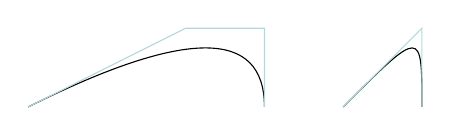
\begin{tikzpicture}
\draw (0,0) .. controls
    (2,1) and (3,1) .. (3,0);
\draw (4,0) .. controls
    (5,1) .. (5,0);
\draw[help lines] (0,0)
    -- (2,1) -- (3,1) -- (3,0)
    (4,0) -- (5,1) -- (5,0);
\end{tikzpicture}
\end{example}

\subsection{绘制二维函数图像}

\begin{figure}[!htb]
    \begin{minipage}[t]{0.5\linewidth}
    \vspace*{0pt}
    如下图,绘制函数图像
    
    \vspace*{1cm}
    \noindent$
    \begin{aligned}
        & y = 2x^2-1\\
        &y = x\\
        & y = \sin(x)\\
        &y = e^x  \\ 
        & \left \{ \begin{matrix} x = 2.5\sin(t)\\ y = 1.5\cos(t)\end{matrix}\right.      
    \end{aligned}
    $ 
    \end{minipage}
    \begin{minipage}[t]{0.5\linewidth}
        \vspace*{0pt}
        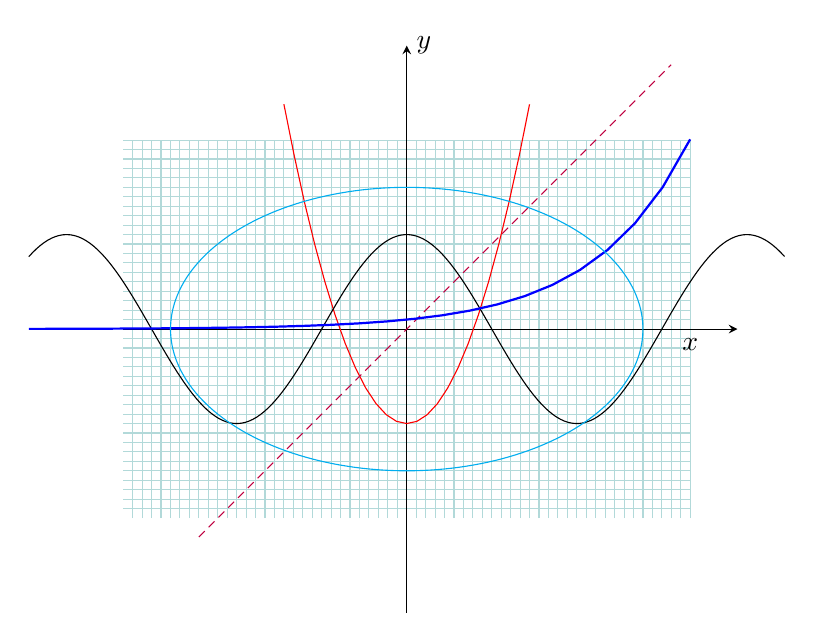
\begin{tikzpicture}[scale=1.2]
            \draw[help lines,step=0.1]
            (-3,-2) grid (3,2);
            % 使用node不方便控制,所以使用coordinate更加的方便
            \draw[-stealth] (-3,0) -- (3.5,0);
            \coordinate[label=right:{$y$}] (y-axis) at (0,3);
            % \node (x) at (3,-0.1) {$x$};      
            \draw[-stealth] (0,-3) -- (0,3);
            \coordinate[label=below:{$x$}] (x-axis) at (3, 0);
            % \node (x) at (0.1, 3) {$y$};
            \draw[domain=-1.3:1.3, red]
                plot(\x, {\x*\x*2 -1});
            \draw[domain=-4:4][samples = 200]       % sample控制描点的个数,使得曲线更加的光滑
                plot(\x, {cos(100*\x)});
            \draw[domain=-2.2:2.8, color=purple, densely dashed][samples = 200]
                plot(\x, {\x});
            \draw[domain=-4:3, color=blue, thick]
                plot(\x, {0.1*exp(\x)});
            % 2. 使用参数方程绘图
            \draw[domain = -2:360, color=cyan][samples = 200] plot({2.5*sin(\x)},{1.5*cos(\x)});
            % 3. Vscode 内置的方式
        \end{tikzpicture}           
    \end{minipage}
\end{figure}
\newpage
% 自定义函数: binom function
\textbf{自定义函数}
\begin{example}
\tikzset{
    declare function={
    binom(\k,\n,\p)=
        \n!/(\k!*(\n-\k)!)*\p^\k*(1-\p)^(\n-\k);
        }
    }
\begin{tikzpicture}[scale=0.7]
    \begin{axis}[samples at={0,...,40},
            yticklabel style={
            /pgf/number format/fixed,
            /pgf/number format/fixed zerofill,
            /pgf/number format/precision=2}
        ]
    \addplot [only marks,orange] {binom(x,40,0.5)};
    \addlegendentry{$p=0.5$}
    \addplot [only marks,cyan] {binom(x,40,0.2)};
    \addlegendentry{$p=0.2$}
    \addplot [smooth,thick,cyan] {binom(x,40,0.2)};
    \addlegendentry{$p=0.2$}
    \end{axis}
\end{tikzpicture}     
\end{example}

    \begin{itemize}
        \item help lines:显示背景网格辅助线
        \item step:domain区间内step参数控制网格大小
        \item domain:函数的绘制区间
    \end{itemize}
    % 4. draw 和 filldraw命令
\subsection{draw 和 filldraw命令}
\begin{example}
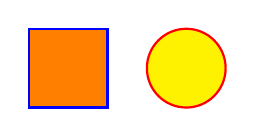
\begin{tikzpicture}[thick]
    \draw[blue, fill=orange] 
        (0,0) rectangle (1,1);
    \filldraw[fill=yellow,draw=red]
        (2,0.5) circle [radius=0.5];
\end{tikzpicture}
\end{example}

\subsection{线条粗细}
\begin{example}
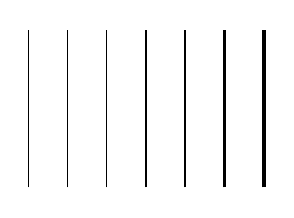
\begin{tikzpicture}
    \draw[ultra thin] (0,0)--(0,2);
    \draw[very thin] (0.5,0)--(0.5,2);
    \draw[thin] (1,0)--(1,2);
    \draw[semithick] (1.5,0)--(1.5,2);
    \draw[thick] (2,0)--(2,2);
    \draw[very thick] (2.5,0)--(2.5,2);
    \draw[ultra thick] (3,0)--(3,2);
\end{tikzpicture}
\end{example}

\subsection{箭头样式}
\begin{example}
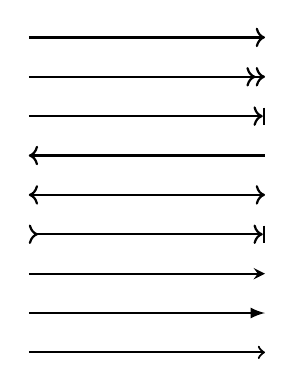
\begin{tikzpicture}[thick]
    \draw[->] (0,4) -- (3,4);
    \draw[->>] (0,3.5) -- (3,3.5);
    \draw[->|] (0,3) -- (3,3);
    \draw[<-] (0,2.5) -- (3,2.5);
    \draw[<->] (0,2) -- (3,2);
    \draw[>->|] (0,1.5) -- (3,1.5);
    \draw[-stealth] (0,1) -- (3,1);
    \draw[-latex] (0,0.5) -- (3,0.5);
    \draw[-to] (0,0) -- (3,0);
\end{tikzpicture} 
\end{example}

\subsection{圆角命令}
\begin{example}
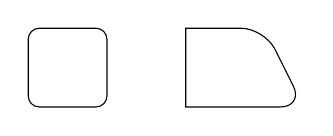
\begin{tikzpicture}
    \draw[rounded corners]
        (0,0) rectangle (1,1);
    \draw (2,0) -- (2,1)
        [rounded corners=.3cm]  % .3 = 0.3
        -- (3,1) -- (3.5,0)
        [sharp corners] -- cycle;
\end{tikzpicture}
\end{example}

\subsection{常见的图形变换}
\begin{example}
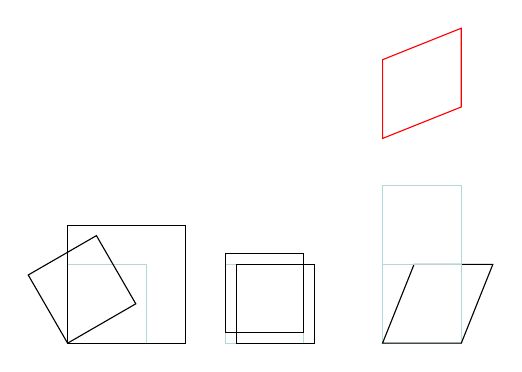
\begin{tikzpicture}
    % help line 参数类似于参考线
    % 变换的图形就是:后边的原始图形
    \draw[help lines](0,0) rectangle (1,1); 
    \draw[scale=1.5] (0,0) rectangle (1,1);
    \draw[rotate=30] (0,0) rectangle (1,1);

    \draw[help lines](2,0) rectangle (3,1);
    \draw[yshift=4pt](2,0) rectangle (3,1);
    \draw[xshift=4pt](2,0) rectangle (3,1);

    % 图形型倾斜
    \draw[help lines](4,0) rectangle (5,1);
    \draw[xslant=0.4](4,0) rectangle (5,1);
    \draw[help lines](4,1) rectangle (5,2);
    \draw[yslant=0.4, red](4,1) rectangle (5,2);
\end{tikzpicture}
\end{example}

\subsection{TikZ的\textcolor{cyan}{样式}概念}

\textbf{1. 在环境外定义}
\begin{example}
% 自定义个样式,只能在最近的一个tikzpicrture中使用
\tikzstyle{bluecircle}=[
    fill={rgb,255: red,137; green,173; blue,255}, 
    draw=red, 
    shape=circle
    ]

% 使用自定义的样式
\begin{tikzpicture}
    \draw[bluecircle] (1, 1) circle [radius=1];
\end{tikzpicture} 
\end{example}

\textbf{2. 在环境内定义}
\begin{example}
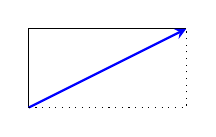
\begin{tikzpicture}
    % 定义样式
    [myarrow/.style={blue,thick,-stealth}] 
    \draw (0,0)--(0,1)--(2,1);
    % 使用样式
    \draw[myarrow] (0,0)--(2,1);
    \draw[dotted] (0,0)--(2,0)--(2,1);
\end{tikzpicture}
\end{example}

\textbf{3. 绘图参数或样式在局部生效}
\begin{example}
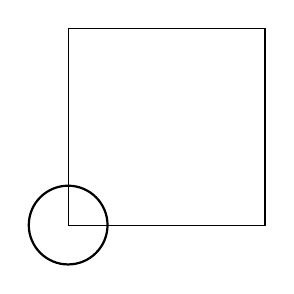
\begin{tikzpicture}
    \draw (0,0) rectangle (2.5, 2.5);
    % 下边这个circle就使用的是局部定义
    \begin{scope}[thick,scale=0.5]
    \draw (0,0) circle [radius=1];
    \end{scope}
\end{tikzpicture}
\end{example}

\subsection{TikZ文字结点}

TikZ用 \cmd{node} 命令绘制文字结点:
\begin{command}
\cmd{node}\oarg{options} \texttt{(\Arg{name})} \texttt{at (\Arg{coordinate})} \marg{text}\texttt{;}
\end{command}
\texttt{(\Arg{name})} 为结点命名,类似 \cmd{coordinate};\texttt{at (\Arg{coordinate})} 指定结点的位置。
这两者和前面的 \Arg{options} 都可以省略,只有 \Arg{text} 是必填的。
\begin{example}
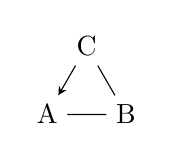
\begin{tikzpicture}
\node (A) at (0,0) {A};
\node (B) at (1,0) {B};
\node (C) at (60:1) {C};
\draw[-stealth] (A) -- (B) -- (C) -- (A);
\end{tikzpicture}
\end{example}

\begin{itemize}
\item \texttt{anchor=\Arg{position}} 令结点的某个角落 \Arg{position} 与 \Arg{coordinate} 对应。
\item \texttt{centered / above / below / left / right / above left / ... \oarg*{=\Arg{length}}} \\
与 \texttt{anchor} 等效的选项。可选的 \Arg{length} 为节点相对于 \Arg{coordinate} 的距离。
\end{itemize}
\begin{example}
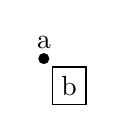
\begin{tikzpicture}
\coordinate (A) at (1,1);
\fill (A) circle[radius=2pt];
% draw选项可以添加一个方框
\node[anchor=south] at (A) {a};
\node[draw,below right=4pt] at (A) {b};
\end{tikzpicture}
\end{example}

\begin{itemize}
\item \texttt{shape=\Arg{shape}}
结点的形状,默认可用 \texttt{rectangle} 和 \texttt{circle},可省略 \texttt{shape=} 直接写。在导言区使用命令
\cmd{use\-tikz\-library}\marg*{shapes.geometric} 可用更多的形状。
\item \texttt{text=\Arg{color}}
结点文字的颜色。
\item \texttt{node font=\Arg{font command}}
结点文字的字体,形如 \cmd{bfseries} 或 \cmd{itshape} 等。
\end{itemize}
\begin{example}
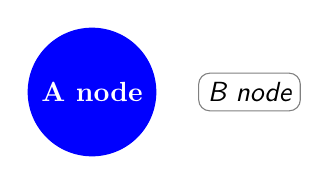
\begin{tikzpicture}
    \node[
        circle,
        fill=blue,
        text=white,
        node font={\bfseries}]
        (A) at (0,0) {A node};

    \node[
        rectangle,
        rounded corners,
        draw=gray,
        node font={\sffamily\slshape}]
        (B) at (2,0) {B node};
\end{tikzpicture}
\end{example}

\textbf{inner \& outer sep参数}
\begin{example}
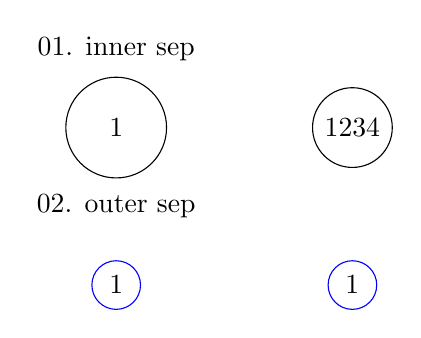
\begin{tikzpicture}
    \node () at (0, 1) {01. inner sep};
    \node[
        circle, 
        draw=black, 
        inner sep=10pt] 
        (node) at (0,0) {1};
    \node[
        circle, 
        draw=black, 
        inner sep=3pt] 
        (node) at (3,0) {1234};

    \node () at (0, -1) {02. outer sep};
    \node[
        circle, 
        draw=blue, 
        outer sep=10pt] 
        (node) at (0,-2) {1};
    \node[
        circle, 
        draw=blue, 
        outer sep=3pt] 
        (node) at (3,-2) {1};
\end{tikzpicture}
\end{example}
\newpage
% 3. 使用tikz定义一个带圈序号命令:无法传参
% 原因:那个默认参数搞的鬼,把呢个默认参数去掉即可。

% 测试
% 经过测试可以在环境定义传入参数
% \newcommand{\test}[1][1]{    
%     \begin{center}
%     #1
%     \end{center}
%     }
% \newcommand{\param}[1]{\ensuremath{\vec{#1}}}
% \newcommand{\testa}[1]{\begin{align}#1\end{align}}
% \test{this is a sentence for test}
% \param{\alpha}
% \testa{\alpha}
\newcommand{\circlenum}[1]{
    \begin{tikzpicture}
        \node[
            circle, 
            draw=black, 
            inner sep=1pt] 
            (node) at (0,0) {\small{#1}};
    \end{tikzpicture}
}
\newcommand{\circlenumnew}[1]{
    \begin{tikzpicture}
        \node[
            circle, 
            draw=black, 
            inner sep=1pt] 
            (node) at (0,0) {\makebox[0.5em][t]{\small#1}};
            % 这里的c, b, t仅仅只是文字的对齐,不是圆圈的对齐
    \end{tikzpicture}
}
% 第二种定义方式
\newcommand{\mycircled}[1]{
    \lower.7ex
    \hbox{
        \tikz\draw (0pt, 0pt) 
        circle(.4em) 
        node{\makebox[0.5em][c]{\small #1}};
        }
}
\begin{example}
\begin{itemize}
    \item 测试文本,Test word:\circlenum{1}
    \item 测试文本,Test word:\circlenum{123456}
    \item 测试文本,Test word:\circlenumnew{1}
    \item 测试文本,Test word:\circlenumnew{123456}
    \item 测试文本,Test word:\mycircled{1}
    \item 测试文本,Test word:\mycircled{123456}
\end{itemize} 
\end{example}


\textbf{标记节点和边的方法}
\cmd{node} 命令的一种等效用法是在 \cmd{draw} 等命令的路径中使用 \texttt{node},不仅可以对某个位置标记节点,还能够对线标记:
\begin{example}
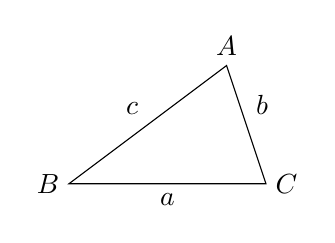
\begin{tikzpicture}
\draw (2,1.5) node[above] {$A$}
       -- node[above left]  {$c$}
      (0,0) node[left]  {$B$}
       -- node[below]       {$a$}
      (2.5,0) node[right] {$C$}
       -- node[above right] {$b$}
       cycle;
\end{tikzpicture}
\end{example}

\section{TiKZ高阶}
\subsection{综合运用}
\begin{example}
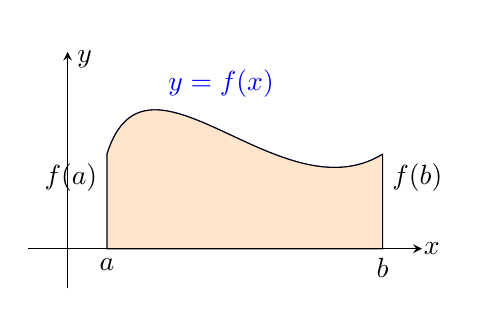
\begin{tikzpicture}
    \draw[-stealth] (-0.5, 0) -- (4.5, 0);
    \node[right] (xaxis) at (4.4, 0) {$x$};
    \draw[-stealth] (0, -0.5) -- (0, 2.5);
    \node[right] (yaxis) at (0, 2.4) {$y$};
    \coordinate (a) at (0.5, 0);
    \coordinate (b) at (4, 0);
    \coordinate (fa) at (0.5, 1.2);
    \coordinate (fb) at (4, 1.2);
    % 一种更简单的确定node位置的方法
    \node[below] at (a |- 0,0) {$a$};
    \node[below] at (b |- 0,0) {$b$};

    % c1, c2 为控制点
    \coordinate (c1) at (1, 2.8);
    \coordinate (c2) at (2.7, 0.4);

    \node[below left] at (fa) {$f(a)$};
    \node[below right] at (fb) {$f(b)$};
    \draw[blue] 
         (fa) .. controls (c1) and (c2) 
              .. node[above=3mm] {$y=f(x)$} (fb); 

    % 开始填充颜色
    % \draw[fill=orange, draw=black] 
    %      (a) -- (fa) -- (fb) -- (b) -- cycle;
    % 01. 填充了一个正方形出来
    % \draw[fill=orange, draw=black] 
    %      (a) -- (fa) .. (fb) -- (b) -- cycle;     
    % 02. --> 报错
    \draw[fill=orange!20, draw=black] 
         (a) -- (fa) .. controls (c1) and (c2) 
                     .. (fb) -- (b) -- cycle;
    % 03. 注意:因为路径是曲线所以你需要在中间使用 ..  
    % 并且输入控制点
    % orange!20: 使用20%的orange
\end{tikzpicture}
\end{example}


\subsection{在TikZ中使用循环}

\cmdindex[tikz]{foreach}
TikZ通过 \pkg{pgffor} 功能宏包实现了简单的循环功能,语法为:
\begin{command}
\cmd{foreach} \cmd{a} \texttt{in} \marg{list} \marg{commands}
\end{command}
上述语法定义了 \cmd{a} 为变量,在 \marg{commands} 中使用 \cmd{a} 完成循环。

\Arg{list} 可以直接将所有值写出来,如 1,2,3,4;也可以写成省略形式,如 1,2,\ldots,10。
\begin{example}
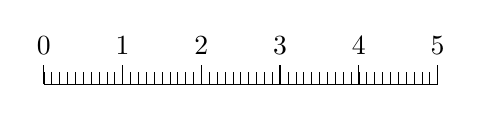
\begin{tikzpicture}
\draw (0,0)--(5,0);
\foreach \i in {0.0,0.1,...,5.0}
  {\draw[very thin]
     (\i,0)--(\i,0.15);}
\foreach \I in {0,1,2,3,4,5}
  {\draw (\I,0)--(\I,0.25)
     node[above] {\I};}
\end{tikzpicture}
\end{example}

\cmd{foreach} 还可使用\textbf{变量对}参与循环, 使用$\mathrm{/}$划分两个变量
\begin{example}
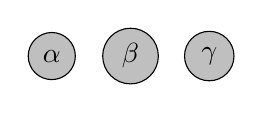
\begin{tikzpicture}
% 这里的变量num表示第几个对象,变量var表示node的内容
\foreach \num/\var in
  {0/\alpha,1/\beta,2/\gamma}
  {\node[circle,fill=lightgray,draw]
    at (\num,0) {$\var$};}
\end{tikzpicture}
\end{example}

\subsection{使用循环绘制一个坐标轴}
\begin{example}
\begin{tikzpicture}
% 1. 标记重要的点
\coordinate (O) at (0, 0);
\coordinate (ymax) at (0, 6);
\coordinate (ymin) at (0, -1.3);
\coordinate (xmax) at (6, 0);
\coordinate (xmin) at (-1.3, 0);

% 2. 绘制基本的坐标轴
\draw[-stealth, thick] (ymin) -- (ymax);
\draw[-stealth, thick] (xmin) -- (xmax);
\node[blue, right=6pt, below] at (ymax) {$y$};
\node[blue, below=6pt, left] at (xmax) {$x$};

% 3. 给x, y轴加上刻度
\node[black, left=8pt, below] at (O) {$O$};
\draw[black] (0, 0.5) -- (0.05, 0.5);
\draw[black] (0.5, 0) -- ( 0.5, 0.05);
\foreach \loc/\x in
    {-1/-1, 1/1, 2/2, 3/3, 4/4, 5/5}
    {\node[blue, below] at (\loc, 0) {$\x$};
     \draw[black, thick] (\loc, 0) -- (\loc, 0.1);
     \draw[black] (\loc+0.5, 0) -- (\loc+0.5, 0.05);
    } 
\foreach \loc/\y in
    {-1/-1, 1/1, 2/2, 3/3, 4/4, 5/5}
    {\node[blue, left] at (0, \loc) {$\y$};
     \draw[black, thick] (0, \loc) -- (0.1, \loc);
     \draw[black] (0, \loc+0.5) -- (0.05, \loc+0.5);
    } 
\end{tikzpicture}
\end{example}


\subsection{使用自定义的坐标轴绘图}
\begin{center}
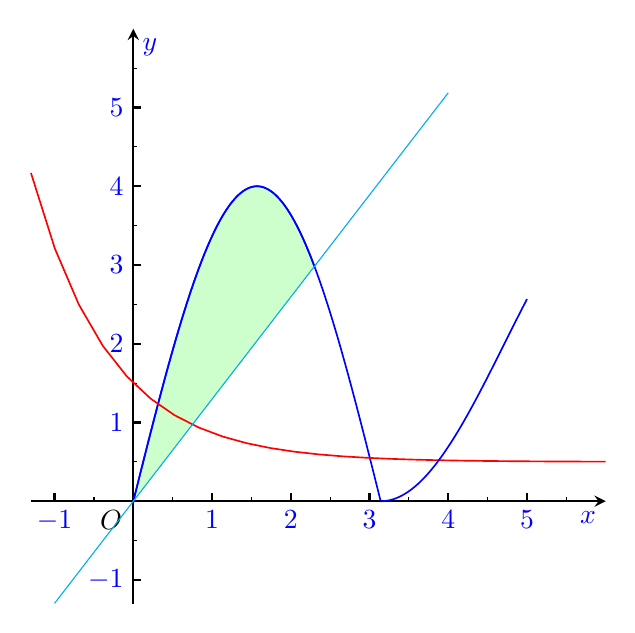
\begin{tikzpicture}{smooth}
% 1. 标记重要的点
\coordinate (O) at (0, 0);
\coordinate (ymax) at (0, 6);
\coordinate (ymin) at (0, -1.3);
\coordinate (xmax) at (6, 0);
\coordinate (xmin) at (-1.3, 0);

% 2. 绘制基本的坐标轴
\draw[-stealth, thick] (ymin) -- (ymax);
\draw[-stealth, thick] (xmin) -- (xmax);
\node[blue, right=6pt, below] at (ymax) {$y$};
\node[blue, below=6pt, left] at (xmax) {$x$};

% 3. 给x, y轴加上刻度
\node[black, left=8pt, below] at (O) {$O$};
\draw[black] (0, 0.5) -- (0.05, 0.5);
\draw[black] (0.5, 0) -- ( 0.5, 0.05);
\foreach \loc/\x in
    {-1/-1, 1/1, 2/2, 3/3, 4/4, 5/5}
    {\node[blue, below] at (\loc, 0) {$\x$};
     \draw[black, thick] (\loc, 0) -- (\loc, 0.1);
     \draw[black] (\loc+0.5, 0) -- (\loc+0.5, 0.05);
    } 
\foreach \loc/\y in
    {-1/-1, 1/1, 2/2, 3/3, 4/4, 5/5}
    {\node[blue, left] at (0, \loc) {$\y$};
     \draw[black, thick] (0, \loc) -- (0.1, \loc);
     \draw[black] (0, \loc+0.5) -- (0.05, \loc+0.5);
    } 
% 4. 绘制函数图
% 使用deg让它认识弧度制
\draw[blue, semithick, domain=0:2.3, fill=green!20][samples=200] plot (\x, {4*sin(deg(\x))});
\draw[blue, semithick, domain=0:pi][samples=200] plot (\x, {4*sin(deg(\x))});
\draw[red, semithick,  domain=-1.3:6] plot(\x, {exp(-\x)+0.5});
\draw[cyan, domain=-1:4] plot(\x,{4*sin(deg(2.3))/2.3*\x});
\draw[blue, semithick, domain=pi:5][samples=200] plot (\x, {2*sin(deg(\x + pi/2))+2});
% \draw [domain=0:1.7, black] (1.7, sin(deg(1.7))) -- (1.7, 0);
% \draw [fill =green!30] 
\end{tikzpicture}
\end{center}

\subsection{函数阴影的填充}
\begin{example}
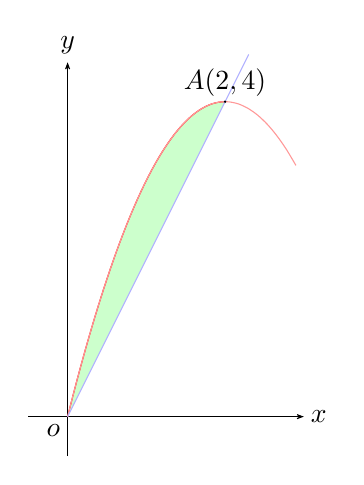
\begin{tikzpicture}[smooth]
    \draw[arrows={-Stealth[length=5pt, inset=3.5pt]}] 
        (-0.5,0) -- (3.0,0)
        node (xaxis) [right=-1pt] {$x$};
    \draw[arrows={-Stealth[length=5pt, inset=3.5pt]}] 
        (0,-0.5) -- (0,4.5)
        node (yaxis) [above=-0.6pt] {$y$};
    \draw  (-0.18,-0.18) node {$o$};
    \draw[color=red,domain=0:2.0,fill=green!20] 
        plot (\x,4*\x-\x*\x);
    \draw[color=red!40,domain=0:2.90] 
        plot (\x,4*\x-\x*\x)  ;
    \draw[color=blue!30,domain=0:2.3] 
        plot (\x,2*\x)  ;
    \draw[fill=black] 
        (2,4) circle [radius=0.2pt] 
        node[above=-1.8pt] {$A(2,4)$};
\end{tikzpicture}
\end{example}


\subsection{封装绘图函数框架}
% 注意:自定义命令中没有前后前后定义的,但是自定义环境有
% \newenvironment{}[][]{}{}
% \newcommand{}[][]{}

\begin{Axis}
    \draw[color=red,domain=0:2.0,fill=green!20] 
        plot (\x, {4*\x-\x*\x});
    \draw[color=blue!30,domain=0:2.3] 
        plot (\x,{ 2*\x});
    \draw[color=black,domain=-1.5:5] 
        plot (\x,{exp(-\x)});  
\end{Axis}
\begin{minipage}[t]{0.5\linewidth}
    \begin{Axis}
        \draw[color=red,domain=1:4.5,fill=blue!20] 
            plot (\x, {4*sin(0.5*\x r)});
        \draw[color=red, thick, domain=-1:4.5] 
            plot (\x,{4.5*(1-\x/4)});
    \end{Axis}
\end{minipage}

\subsection{图形的填充}
\begin{itemize}
    \item 1. 类似2.13中的把曲线画出来:控制点已知
    \item 2. 类似2.17默认是(0, 0) - - f(x) - - f(xmax) - - (0, 0) 的路径。
    \item 3. 把2. 中的(0, 0) $\rightarrow$ (a, b)
\end{itemize}

\subsection{TiKZ小技巧}
\begin{itemize}
    \item 1. >=stealth: 指定局部的范围(tikzpicture)的箭头样式
    \item 2. 填充样式的宏包:$\backslash$usetikzlibrary\{patterns\}。比如$\backslash$draw[pattern=north east lines] $\cdots$
    \item 3. node节点样式的另外一种格式:
            $\backslash$node ($s_1$) at (0, 0)[rectangle, draw=black, fill=blue] \{example text\}
    \item 4. 三角函数默认使用度数绘图:使用sin(deg(x)), sin($\backslash$x r).(x为弧度)
    \item 5. node的命名(如$s_1$)可用变量实现:$\backslash$node (s$\backslash$x) at $\cdots$(其中$\backslash$x是$\in$\{1, 2, 3\}中的变量)
    \item 6. bend命令可以实现直线的弯曲(角度)命令:$\backslash$draw[->] to [bend left=25] $\cdots$
    \item 7. 可以在draw的同时就把node给标注了$\backslash$draw (140:1)node[left]\{node1\} - - (0, 0) - - (97.2:1);
\end{itemize}
\newpage
\subsection{坐标重置}
\begin{center}

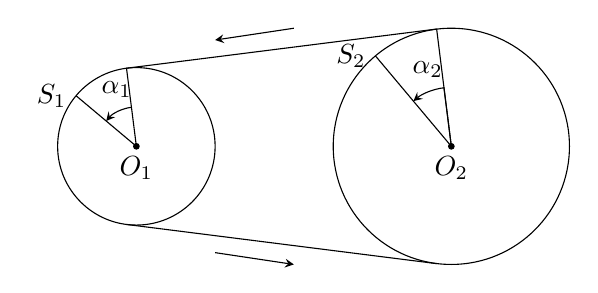
\begin{tikzpicture}[>=stealth]
\draw (0, 0) circle(1);
\draw (4, 0) circle(1.5);
\draw[fill=black] (0, 0) circle(1pt);
\draw[fill=black] (4, 0) circle(1pt);

\node[below] (O1) at (0, 0) {$O_1$};
\node[below] (O2) at (4, 0) {$O_2$};

%% 使用角度来找几何关系绘图(极坐标)
%% (a, b) --+ (c, d) : 表示把(a, b)看作坐标原点,或者说是后边邻近的坐标(c, d)是相对于(a, b)的相对坐标
\draw (140:1)node[left]{$S_1$} 
   -- (0, 0) 
   -- (97.2:1) 
   --+ (7. 2:3.97) 
   -- (4, 0) 
   --+ (130:1.5)node[left]{$S_2$};

%% 下边对称的直线只需符号取反即可。
\draw (-97.2:1) 
  --+ (-7. 2:3.97); 

%% 绘制圆弧arch命令
\draw[->] (97.2:0.5) arc (97.2:140:0.5); 
%% 下边由于O2不是原点,所以我们的想办法把它变为原点,这样就可以用arch方便的绘图
\draw[->] (4, 0) --+ (97.2:0.75) arc (97.2:130:0.75);
%% (4, 0) --+ (97.2:0.75): 这条线覆盖了原来的线

%% 直接使用坐标定位绘制剩余的标注
\node at (-0.25, 0.5)[above]{$\alpha_1$};
\node at (4-0.3, 0.75)[above]{$\alpha_2$};
\draw[<-] (1, 1.35) -- (2, 1.5);
\draw[->] (1, -1.35) -- (2, -1.5);
\end{tikzpicture}  
  
\end{center}
%% 1. 给每一个子图指定一个相对坐标
%% 2. 使用scope分出三个区域。scope默认居中,所以需要平移一段距离--> xshift
%% 3. 相当于每一个scope范围都是一个独立的坐标系统,都有一个独立的坐标原点

\subsection{多图排版}

\begin{tikzpicture}[>=stealth]
%% 第一个区域
\begin{scope}
    \draw [->] (-1.5, 0) -- (1.5, 0)node [right] {$x$};
    \draw [->] (0, -1.5) -- (0, 1.5)node [right] {$y$};
    \draw (0, 0) circle(1);
    \node at (-0.25, -0.25) {$O$};

    %% 循环内部用{}不是(): 原因:LaTeX的宏替换机制{}内部是一个整体,不能分割。
    \foreach \x/\xcorr in {+/{0.5, 0.5}, -/{-0.5, 0.5}, -/{-0.5, -0.5}, +/{0.5, -0.5}}
    {
        \node at (\xcorr) {$\x$};
    }
    \node at (0, -2) {$\cos\alpha$和$\sec\alpha$};
\end{scope}

%% 第二个区域
\begin{scope}[xshift=6cm]
    \draw [->] (-1.5, 0) -- (1.5, 0)node [right] {$x$};
    \draw [->] (0, -1.5) -- (0, 1.5)node [right] {$y$};
    \draw (0, 0) circle(1);
    \node at (-0.25, -0.25) {$O$};

    \foreach \x/\xcorr in {+/{0.5, 0.5}, +/{-0.5, 0.5}, -/{-0.5, -0.5}, -/{0.5, -0.5}}
    {
        \node at (\xcorr) {$\x$};
    }
    \node at (0, -2) {$\sin\alpha$和$\csc\alpha$};
\end{scope}

%% 第三个区域
\begin{scope}[xshift=12cm]
    \draw [->] (-1.5, 0) -- (1.5, 0)node [right] {$x$};
    \draw [->] (0, -1.5) -- (0, 1.5)node [right] {$y$};
    \draw (0, 0) circle(1);
    \node at (-0.25, -0.25) {$O$};

    \foreach \x/\xcorr in {+/{0.5, 0.5}, -/{-0.5, 0.5}, +/{-0.5, -0.5}, -/{0.5, -0.5}}
    {
        \node at (\xcorr) {$\x$};
    }
    \node at (0, -2) {$\tan\alpha$和$\cot\alpha$};
\end{scope}

\end{tikzpicture}
\subsection{圆柱体等三维图形的绘制}

%% 核心思想还是三维图形的二维坐标化
\begin{example}
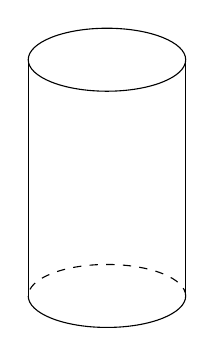
\begin{tikzpicture}
\draw (-1, 0) -- (-1, 3);
\draw (1,0) -- (1, 3);

%% 绘制椭圆
\draw (0, 3) ellipse [x radius=1, y radius=0.4];
% \draw (0, 0) ellipse [x radius=1, y radius=0.4];
\draw[dashed] (1, 0) arc [start angle=0, 
                          end angle=180, 
                          x radius=1, 
                          y radius=0.4];
\draw (1, 0) arc [start angle=0, 
                  end angle=-180, 
                  x radius=1, 
                  y radius=0.4];
\end{tikzpicture}    
\end{example}

\subsection{平面几何宏包}

%% 一些平面几何使用的宏包\
%% 代码后边不用加;也可以加分号
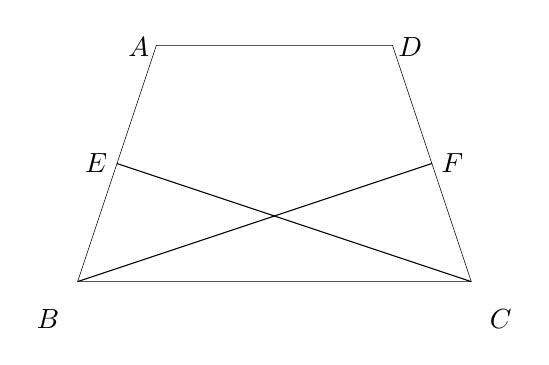
\begin{tikzpicture}

% 定义多个点(a/b/<name>):坐标(a, b), 名称<name>
\tkzDefPoints{-2.5/0/B, 2.5/0/C, -1.5/3/A, 1.5/3/D, 0/1.5/O}
%% 调用Euclide包中的函数进行操作:求中点, 垂线 ……

%% 定义一个点-->中间不能加空格(A, B)会报错        得到这个点(设为变量E)
\tkzDefMidPoint(A,B)   \tkzGetPoint{E}
\tkzDefMidPoint(C,D)   \tkzGetPoint{F}

%% 连接点
\tkzDrawPolygon(A, B, C, D)

%% 可以使用tikz命令来连接euclide定义的点, 它们二者兼容
\draw (B) -- (F)node[right]{$F$};
\draw (C) -- (E)node[left]{$E$};

%% 以O为中心自动填充标签ABCD。不用加$$
\tkzAutoLabelPoints[center=O](A,B,C,D) 

\end{tikzpicture}

\textbf{一个完美的应用}
\begin{example}
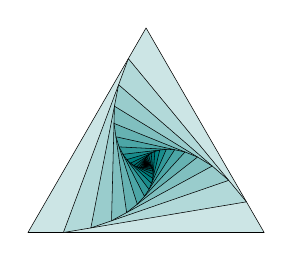
\begin{tikzpicture}[scale=.25]
\tkzDefPoints{00/0/A,12/0/B,6/12*sind(60)/C}
\foreach \density in {20,30,...,240}{%
\tkzDrawPolygon[fill=teal!\density](A,B,C)
\pgfnodealias{X}{A}
\tkzDefPointWith[linear,K=.15](A,B) \tkzGetPoint{A}
\tkzDefPointWith[linear,K=.15](B,C) \tkzGetPoint{B}
\tkzDefPointWith[linear,K=.15](C,X) \tkzGetPoint{C}}
\end{tikzpicture}    
\end{example}

\begin{example}
\begin{tikzpicture}[scale=.75,rotate=-30]
\tkzDefPoint(0,0){O}
\tkzDefPoint(4,-5){A}
\tkzDefIntSimilitudeCenter(O,3)(A,1)
\tkzGetPoint{I}
\tkzExtSimilitudeCenter(O,3)(A,1)
\tkzGetPoint{J}
\tkzDefTangent[from with R= I](O,3 cm)
\tkzGetPoints{D}{E}
\tkzDefTangent[from with R= I](A,1 cm)
\tkzGetPoints{D'}{E'}
\tkzDefTangent[from
with R= J](O,3 cm)
\tkzGetPoints{F}{G}
\tkzDefTangent[from with R= J](A,1 cm)
\tkzGetPoints{F'}{G'}
\tkzDrawCircle[R,fill=red!50,opacity=.3](O,3 cm)
\tkzDrawCircle[R,fill=blue!50,opacity=.3](A,1 cm)
\tkzDrawSegments[add = .5 and .5,color=red](D,D' E,E')
\tkzDrawSegments[add= 0 and 0.25,color=blue](J,F J,G)
\tkzDrawPoints(O,A,I,J,D,E,F,G,D',E',F',G')
\tkzLabelPoints[font=\scriptsize](O,A,I,J,D,E,F,G,D',E',F',G')
\end{tikzpicture}
\end{example}

\begin{example}
\begin{tikzpicture}[scale=.8]
    \tkzDefPoint(3,3){c}
    \tkzDefPoint(6,3){a0}
    \tkzRadius=1 cm
    \tkzDrawCircle[R](c,\tkzRadius)
    \foreach \an in {0,10,...,350}{
    \tkzDefPointBy[rotation=center c angle \an](a0)
    \tkzGetPoint{a}
    \tkzDefTangent[from with R = a](c,\tkzRadius)
    \tkzGetPoints{e}{f}
    \tkzDrawLines[color=magenta](a,f a,e)
    \tkzDrawSegments(c,e c,f)
    }%
\end{tikzpicture}
\end{example}

\begin{example}
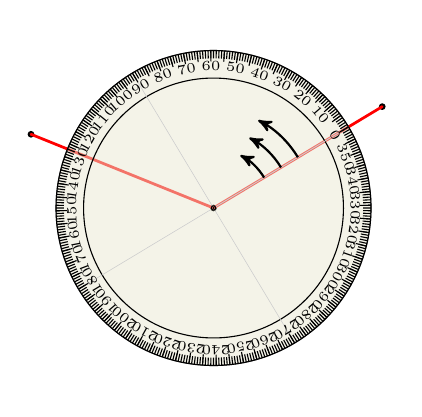
\begin{tikzpicture}[scale=.5]
\tkzDefPoint(2,0){A}\tkzDefPoint(0,0){O}
\tkzDefShiftPoint[A](31:5){B}
\tkzDefShiftPoint[A](158:5){C}
\tkzDrawPoints(A,B,C)
\tkzDrawSegments[color = red,
line width = 1pt](A,B A,C)
\tkzProtractor[scale = 1](A,B)
\end{tikzpicture}
\end{example}

\section{TiKZ in mathcha}
\tikzset{every picture/.style={line width=0.75pt}} %set default line width to 0.75pt        

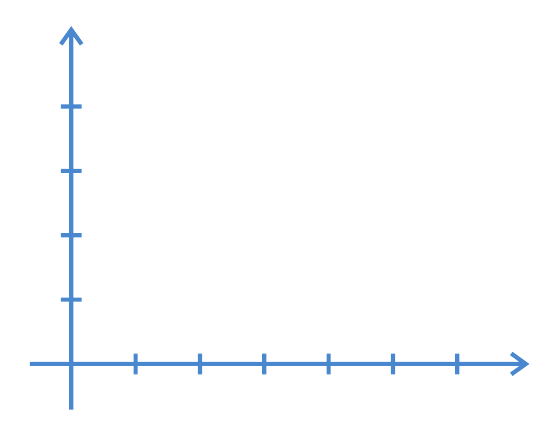
\begin{tikzpicture}[x=0.75pt,y=0.75pt,yscale=-1,xscale=1]
%uncomment if require: \path (0,235); %set diagram left start at 0, and has height of 235

%Shape: Axis 2D [id:dp048941842347560494] 
\draw [color={rgb, 255:red, 73; green, 135; blue, 206 }  ,draw opacity=1 ][line width=1.5]  (41,177) -- (280,177)(61,16) -- (61,199) (273,172) -- (280,177) -- (273,182) (56,23) -- (61,16) -- (66,23) (92,172) -- (92,182)(123,172) -- (123,182)(154,172) -- (154,182)(185,172) -- (185,182)(216,172) -- (216,182)(247,172) -- (247,182)(56,146) -- (66,146)(56,115) -- (66,115)(56,84) -- (66,84)(56,53) -- (66,53) ;
\draw   ;




\end{tikzpicture}
\end{document}


